\documentclass{article}
\usepackage{amsmath,amssymb,amsthm}
\usepackage{fancyhdr}
\usepackage{enumerate}
\usepackage[ruled]{algorithm2e}
\usepackage{tikz}
\usetikzlibrary{arrows.meta}

\pagestyle{fancy}
\fancyhf{}
\lhead{8th Homework - CSCE 411 700}
\rhead{Kevin Lei}
\renewcommand{\headrulewidth}{0.4pt}
\renewcommand{\arraystretch}{1.2}

\newtheorem{theorem}{Theorem}

\begin{document}

\section{Main Idea}

In this problem, we have athletes from $n$ countries participating in $m$ games at the 2020 Olympics.
We denote $C = \{c_1, c_2, \ldots, c_n\}$ as the set of $n$ countries and $H = \{h_1, h_2, \ldots, h_m\}$ as the set of $m$ games.
We assume for simplicity that each country sends at most one athlete to each game, and each game has at least three countries participating.
Let $A_i \subseteq C$ for $i = 1, 2, \ldots, m$ be the set of countries participating in game $h_i$.
Each game produces three medals: gold, silver, and bronze.
Let $x_j$ for $j = 1, 2, \ldots, n$ be the number of medals won by country $c_j$.
The goal is to determine if some arbitrary vector $X = (x_1, x_2, \ldots, x_n)$ is a possible outcome of the 2020 Olympics.

This problem can be modeled as a maximum flow problem.
We can construct a flow network where the maximum flow corresponds to a valid medal distribution.
Let there be a source node $s$ and a sink node $t$.
We create a node $c_j$ for each country, and it is connected to the source with a capacity of $x_j$.
Create nodes $h_i$ for each game, and connect it to each country in $A_i$ with a capacity of 1.
Finally, connect each game node to the sink with a capacity of 3.

\begin{figure}[h]
    \centering
    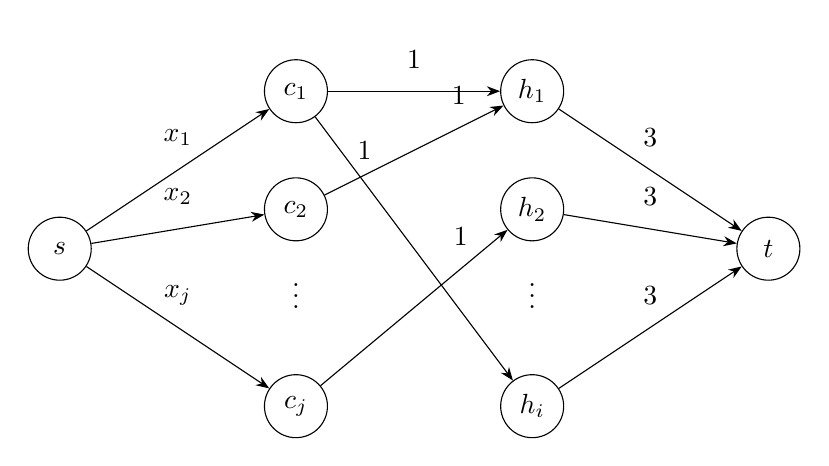
\begin{tikzpicture}[
        node distance=2cm and 3cm,
        every node/.style={circle, draw, minimum size=0.8cm},
        >=Stealth
    ]
        \node (s) at (0,0) {$s$};
        \node (c1) at (3,2) {$c_1$};
        \node (c2) at (3,0.5) {$c_2$};
        \node (cj) at (3,-2) {$c_j$};
        \node (h1) at (6,2) {$h_1$};
        \node (h2) at (6,0.5) {$h_2$};
        \node (hi) at (6,-2) {$h_i$};
        \node (t) at (9,0) {$t$};

        \draw[->] (s) -- node[midway, above, draw=none] {$x_1$} (c1);
        \draw[->] (s) -- node[midway, above, draw=none] {$x_2$} (c2);
        \draw[->] (s) -- node[midway, above, draw=none] {$x_j$} (cj);

        \draw[->] (c1) -- node[midway, above, draw=none] {1} (h1);
        \draw[->] (c1) -- node[near start, above, draw=none] {1} (hi);
        \draw[->] (c2) -- node[near end, above, draw=none] {1} (h1);
        \draw[->] (cj) -- node[near end, above, draw=none] {1} (h2);

        \draw[->] (h1) -- node[midway, above, draw=none] {3} (t);
        \draw[->] (h2) -- node[midway, above, draw=none] {3} (t);
        \draw[->] (hi) -- node[midway, above, draw=none] {3} (t);

        \node[draw=none] at (3,-0.5) {$\vdots$};
        \node[draw=none] at (6,-0.5) {$\vdots$};
    \end{tikzpicture}
    \caption{Flow network for the 2020 Olympics}
\end{figure}

We then find the maximum flow using the Ford-Fulkerson algorithm.
If the maximum flow is equal to the total number of medals (i.e. $3m$), then $X$ is a possible outcome of the 2020 Olympics.


\section{Pseudocode}

\begin{algorithm}[H]
    \caption{Check possible outcome}
    \KwIn{Vector of outcomes $X$, set of $n$ countries $C$, set of $m$ games $H$}
    \KwOut{True if $X$ is a possible outcome, False otherwise}
    \BlankLine
    Initialize flow network $G = (V, E)$ as described above\;
    $totalMedals = 3m$\;
    $maxFlow = 0$\;
    \While{there exists an augmenting path $p$ from $s$ to $t$ in the residual graph $G_f$}{
        $c_f = \min\{c_f(u,v) \mid (u,v) \in p\}$\;
        \For{each edge $(u,v) \in p$}{
            \If{$(u,v)$ is a forward edge}{
                $f(u,v) = f(u,v) + c_f$\;
            }
            \Else{
                $f(v,u) = f(v,u) - c_f$\;
            }
        }
        $maxFlow = maxFlow + c_f$\;
    }
    \If {$maxFlow = totalMedals$}{
        \Return True\;
    }
    \Return False\;
\end{algorithm}

\section{Proof of Correctness}

\begin{proof}
    $(\Rightarrow)$ Assume the algorithm retuns true.
    That means we have found a maximum flow equal to the total number of medals.
    That implies the following:
    \begin{itemize}
        \item All game nodes $h_i$ both send and receive 3 units of flow.
        \item Each country node $c_j$ sends $x_j$ units of flow.
        \item Country nodes send either 0 or 1 unit of flow to game nodes.
    \end{itemize}
    Each game node sending 3 units of flow implies that the game results in 3 medals.
    Each country sending $x_j$ units of flow implies that country $c_j$ won exactly $x_j$ medals.
    Finally, since each country sends either 0 or 1 unit of flow to game nodes, each country participates in at most one game.
    Therefore, when the algorithm returns true, the flow network corresponds to a valid medal distribution.
    \vspace{1em}

    \noindent $(\Leftarrow)$ Assume that $X$ is a possible outcome of the 2020 Olympics.
    Then there exists a flow network that corresponds to the medal distribution with the constraints.
    For each medal won by country $c_j$, we send $x_j$ units of flow from $s$ to $c_j$.
    By construction, this flow satisfies the capacity constraints.
    The total flow will be the maximum flow, which is equal to the total number of medals.
    Thus the algorithm is correct.
\end{proof}

\section{Runtime Analysis}

The majority of this algorithm is the Ford-Fulkerson algorithm.
However, first we need to construct the flow network.
Graph construction can be done in $O(n + m + |A|)$ time, where $|A|$ is the total number of participations in all games.
In the Ford-Fulkerson algorithm, the number of iterations is bounded by the maximum flow value, i.e. $3m$.
In each iteration, finding an augmenting path takes $O(V + E)$ time.
Since the flow network has $|V| = n + m + 2$ and $|E| \leq n + |A| + m$, the time complexity of the algorithm is $O(3m(n + m + |A|))$.

\end{document}